% !TEX TS-program = lualatex
%\documentclass[handout]{beamer}
\documentclass{beamer}
\input{../common/misomva}
\newcommand{\misoclasstinytitleslide}{Partially based on material by:  Ulrike von Luxburg, Mikhail Belkin, Partha Niyogi, \\[-1em] Olivier Chapelle, Bernhard Sch\"olkopf, Gary Miller, Doyle \& Schnell, Daniel Spielman}
\newcommand{\misoclassdate}{}
\usetikzlibrary{graphs}

\begin{document}
% Topic-specific title slide
\newcommand{\topictitle}{Manifold Learning}
\newcommand{\topicsubtitle}{Laplacian Eigenmaps}

\MakeTopicSlide

\begin{frame}
\frametitle{Background: Manifold Learning}

\begin{block}{problem: definition reduction/manifold learning}
Given $\{\bx_i\}_{i=1}^\nodes$ from $\R^d$ find $\{\by_i\}_{i=1}^\nodes$
in $\R^m$, where $m \ll d$.
\end{block} 
\pause
\begin{itemize}[<+-| alert@+>]%\addtolength{\itemsep}{0.25\baselineskip}
\item \questionbox{What do we know about the \gcol{dimensionality reduction}}
\begin{itemize}
\item representation/visualization (2D or 3D)
\item an old example: globe to a map
\item often assuming ${\cal M} \subset \R^d$
\item feature extraction
\item linear vs.\,nonlinear dimensionality reduction
\end{itemize}
\item \questionbox{What do we know about linear vs.\@ nonlinear methods?}
\begin{itemize}[<+-| alert@+>]%\addtolength{\itemsep}{0.25\baselineskip}
\item linear: ICA, PCA, SVD, \dots
\item nonlinear often preserve only \gcol{local} distances
\end{itemize}
\end{itemize}

\end{frame}



%%%%%%%%%%%%%%%%%%%%%%%%%%%%%%%%%%%%%%%%%%%%%%%%%%%%%%%%%%%%
\begin{frame}
\frametitle{Manifold Learning: Linear vs. Non-linear}
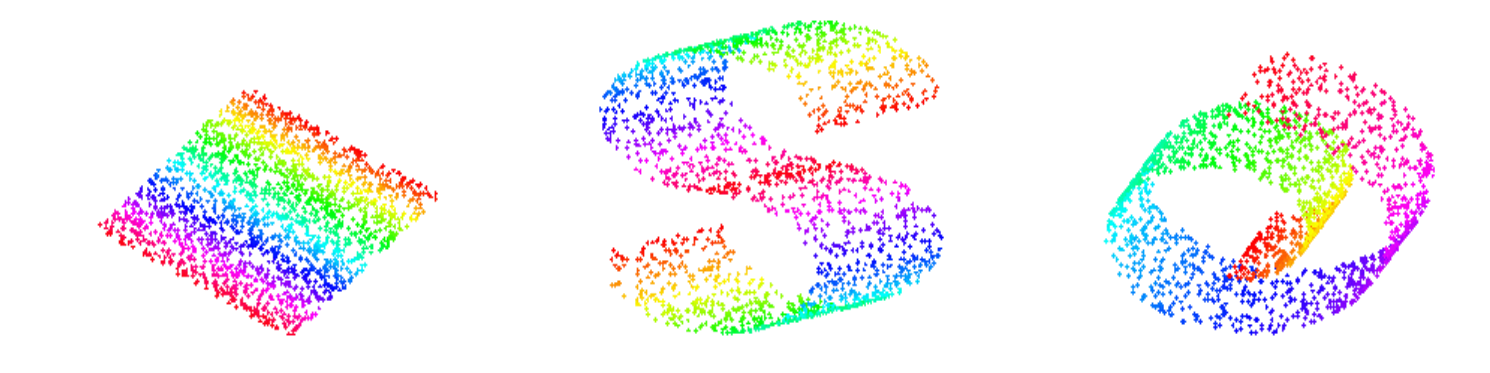
\includegraphics[width=\columnwidth]{../img/manifolds}
\\
{\tiny Source: Belkin \& Niyogi (2003)}
\end{frame}
%%%%%%%%%%%%%%%%%%%%%%%%%%%%%%%%%%%%%%%%%%%%%%%%%%%%%%%%%%%%
\begin{frame}
\frametitle{Manifold Learning: Linear vs. Non-linear (Alternative View)}
\begin{center}
\questionbox{What do we know about linear vs.\@ nonlinear methods?}
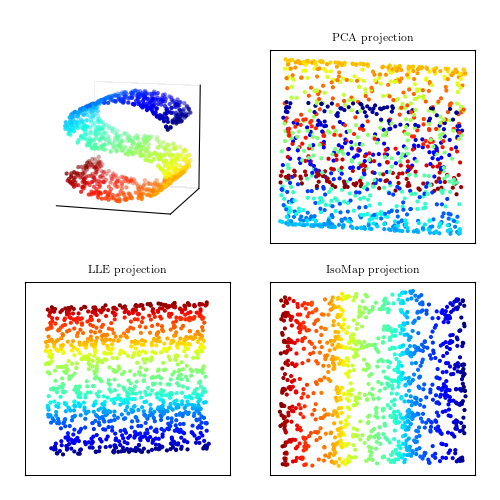
\includegraphics[width=.65\columnwidth]{../img/linear_vs_nonlinear.png}
\\
{\tiny Source: Belkin \& Niyogi (2003)}
\end{center}
\end{frame}
%%%%%%%%%%%%%%%%%%%%%%%%%%%%%%%%%%%%%%%%%%%%%%%%%%%%%%%%%%%%
\begin{frame}
\frametitle{Manifold Learning: Preserving (just) local distances}
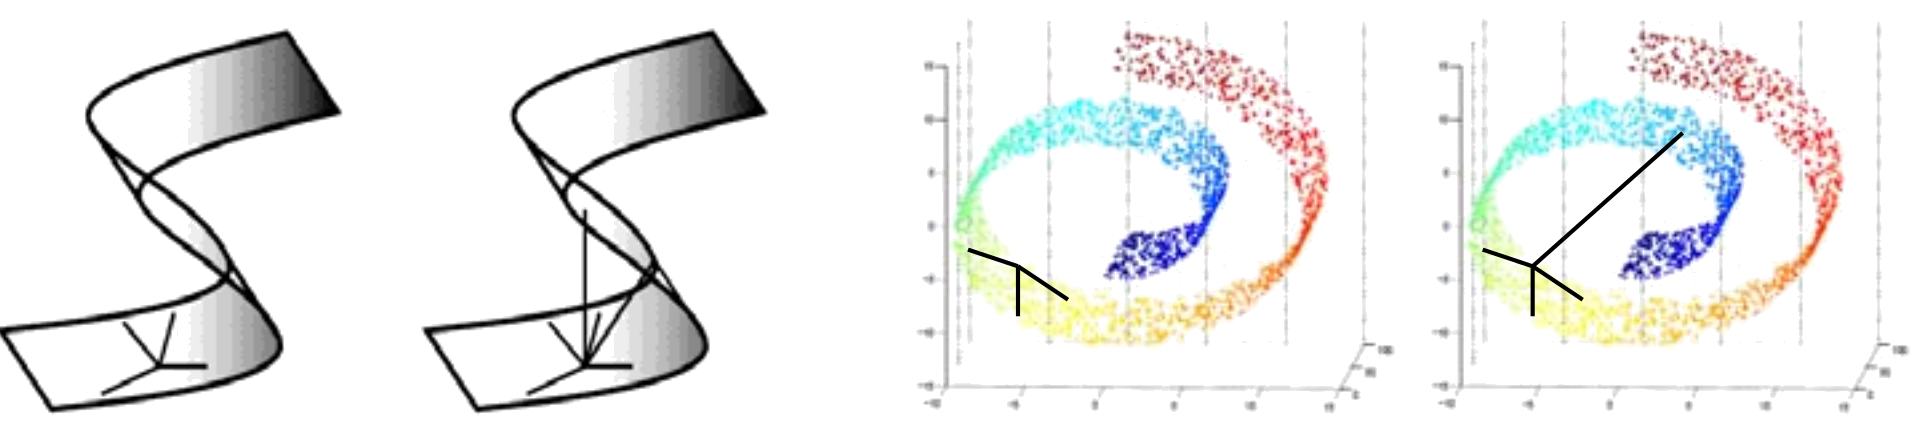
\includegraphics[width=\columnwidth]{../img/manifolds1}
\\
{\tiny Source: Belkin \& Niyogi (2003)}
\pause 
\[
 d(\by_i,\by_j) = d(\bx_i,\bx_j) 
\mbox{\quad only if \quad} 
d(\bx_i,\bx_j)
\mbox{\quad is small} 
\]
\pause 
\[
\text{1-D} \quad\quad\quad \min_{y} \sum_{ij} w_{ij} ( y_i - y_j )^2
\]
\pause 
\[
m\text{-D} \quad\quad\quad \min_{\by} \sum_{ij} w_{ij} \| \by_i - \by_j \|^2
\]
\pause 
\begin{center}
 \questionbox{Looks familiar?}
\end{center}

\end{frame}
%%%%%%%%%%%%%%%%%%%%%%%%%%%%%%%%%%%%%%%%%%%%%%%%%%%%%%%%%%%%
\begin{frame}
\frametitle{Manifold Learning: Laplacian Eigenmaps}

\textbf{Step 1:} Solve generalized eigenproblem: 
\[
  \bL \bff = \lambda \bD \bff
\]

\pause
\textbf{Step 2:} Assign $m$ new coordinates: 
\[
 \bx_i \mapsto \left(f_2\left(i\right), \dots, f_{m+1}\left(i\right)\right) = \by_i
\]
\pause
\textbf{Note$_1$:} we need to get $m+1$ smallest eigenvectors \\
\pause
\textbf{Note$_2$:} $\bff_1$ is useless  \\
\bigskip

{\scriptsize 
\url{http://web.cse.ohio-state.edu/~mbelkin/papers/LEM_NC_03.pdf}
} 

\end{frame}
%%%%%%%%%%%%%%%%%%%%%%%%%%%%%%%%%%%%%%%%%%%%%%%%%%%%%%%%%%%%
\begin{frame}
\frametitle{Manifold Learning: Laplacian Eigenmaps to 1D}

\begin{block}{\centering Laplacian Eigenmaps 1D objective}
\[  
\min_{\bff} \bff \transpose  \bL \bff \quad {\rm s.t.} 
\quad f_i \in \R,
\quad \bff \transpose \bD \bOne = 0, 
\quad \bff \transpose \bD \bff = \bOne
\]
\end{block} 
\pause \bigskip
The meaning of the constraints is similar as for spectral clustering: \\
\bigskip
$\bff \transpose \bD \bff = \bOne$ is for \pause scaling \pause \\
\bigskip
$\bff \transpose \bD \bOne = 0$ is to \pause not get $\bv_1$ \pause \\
\bigskip
\questionbox{What is the solution?}
\end{frame}
%%%%%%%%%%%%%%%%%%%%%%%%%%%%%%%%%%%%%%%%%%%%%%%%%%%%%%%%%%%%

\begin{frame}
\frametitle{Manifold Learning: Example}
\begin{center}
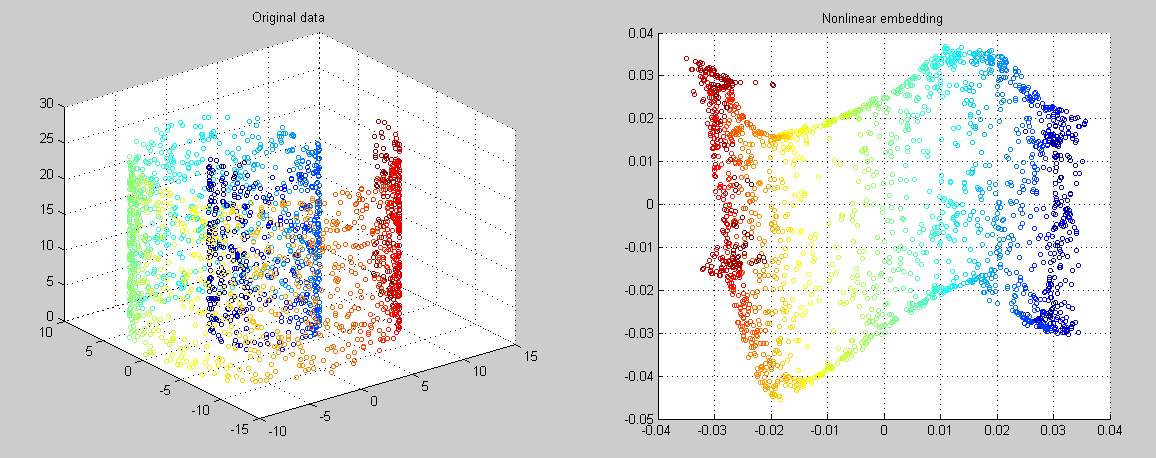
\includegraphics[width=\columnwidth]{../img/laplacianeigenmaps} \\
\bigskip
{\tiny Source: Belkin \& Niyogi (2003); MATLAB implementation: \url{http://www.mathworks.com/matlabcentral/fileexchange/36141-laplacian-eigenmap-~-diffusion-map-~-manifold-learning}}
\end{center}

\end{frame}


\MakeLastSlide
\end{document}
